\documentclass[11pt,a4paper]{article}

\usepackage[margin=1.8cm]{geometry}
\usepackage{booktabs}
\usepackage{array}
\usepackage{longtable}
\usepackage{enumitem}
\usepackage{needspace}
\usepackage{xcolor}
\usepackage{fancyhdr}
\usepackage{pdflscape}
\usepackage{listings}
\usepackage{caption}
\usepackage{tikz}
\usepackage{pdflscape}
\usetikzlibrary{shapes.geometric, positioning}
\usetikzlibrary{shapes.geometric, positioning}
\usepackage[hidelinks]{hyperref}

\definecolor{maroon}{RGB}{110,30,30}

\newcommand{\cl}[1]{\texttt{\detokenize{#1}}}
\newcommand{\pk}[1]{\underline{\texttt{\detokenize{#1}}}}

\setlength{\parindent}{0pt}
\setlength{\emergencystretch}{4em}
\tolerance=2000
\setlength{\parskip}{6pt}
\renewcommand{\arraystretch}{1.25}
\setlist{itemsep=2pt,topsep=3pt}

\pagestyle{fancy}
\fancyhf{}
\lhead{VibeCheck -- DBMS Laboratory Mini-Project}
\rhead{\thepage}
\renewcommand{\headrulewidth}{0.4pt}
\setlength{\headheight}{14pt}

\lstset{
  language=SQL,
  basicstyle=\ttfamily\footnotesize,
  keywordstyle=\bfseries,
  breaklines=true,
  frame=single,
  framerule=0.3pt,
  xleftmargin=2pt,
  xrightmargin=2pt,
  aboveskip=6pt,
  belowskip=6pt
}

\begin{document}

%% ------------------------------------------------------------------ cover
\begin{titlepage}
\thispagestyle{empty}
\centering

\vspace*{2.5cm}

{\huge Database Management Systems Laboratory\par}
\vspace{0.6cm}
{\LARGE Mini-Project Report\par}

\vspace{1.8cm}

% Box containing project title and description
\noindent\fbox{%
    \parbox{\dimexpr\linewidth-2\fboxsep-2\fboxrule\relax}{%
        \centering
        \vspace{0.5cm}
        {\Huge\bfseries VibeCheck\par}
        \vspace{0.3cm}
        {\Large Audio Recognition and Discovery System\par}
        \vspace{0.5cm}
    }%
}\par

\vspace{2.2cm}

{\large Submitted by\par}
\vspace{0.4cm}

\begin{tabular}{|l|l|}
\hline
\textbf{MIS No.} & \textbf{Name} \\
\hline
612415061 & Bhavesh Gadling \\
\hline
612415070 & Jibran Jamdar \\
\hline
612415095 & Sangram Lohokare \\
\hline
\end{tabular}

\vfill

{\large October 2026\par}

\end{titlepage}
\tableofcontents
\newpage

%% ------------------------------------------------------------------ 1
\section{Problem Statement}

People often hear a song in a caf\'e, in a film or on another device and want to know its title and artist immediately. Searching by half-remembered lyrics is slow and often fails. This project builds a small database application that listens to a few seconds of audio and tells the user which song is playing, along with its artist, genre and release year.

Audio cannot be compared sample by sample, because a phone recording differs from the original in loudness, background noise and starting point. The system therefore converts audio into an \emph{audio fingerprint}: a set of integer hashes, each derived from a pair of spectral peaks, together with the time at which the pair occurs in the song. The fingerprints of every song known to the system are stored in a relational database. A recording is identified by looking up its hashes in the database and checking which song has many matching hashes that line up consistently in time. The identified song is saved in the user's recognition history.

The database problem is therefore to store a catalogue of songs, artists, genres, users and recognition history, together with a large table of fingerprints, so that a short noisy clip can be matched to the right song quickly while all data stays consistent.

%% ------------------------------------------------------------------ 2
\section{Objectives}

\begin{enumerate}
  \item Design a relational database for users, songs, artists, genres, audio fingerprints and recognition history, normalized up to Third Normal Form.
  \item Store fingerprints in a way that makes matching fast, using a B-Tree index on the hash column.
  \item Maintain data integrity with primary keys, foreign keys, unique and check constraints, and cascading deletes.
  \item Keep derived data consistent automatically using a trigger, and make every recognition an atomic transaction.
  \item Provide database views that hide joins and aggregation, so the application reads song details and user history with a simple query.
  \item Build a working front end (mobile app) and back end (REST API) on top of the database, so the design is tested by a real application.
\end{enumerate}

%% ------------------------------------------------------------------ 3
\section{Functional Requirements}

\subsection{Functional requirements}


\begin{longtable}{|p{1.5cm}|p{14cm}|}
\hline
\textbf{ID} & \textbf{Requirement} \\
\hline
\endfirsthead

\hline
\textbf{ID} & \textbf{Requirement} \\
\hline
\endhead

FR1 & A new user can register with first name, optional middle and last name, e-mail address and password. \\
\hline
FR2 & A registered user can log in with e-mail and password and receives an authentication token. \\
\hline
FR3 & A logged-in user can record about six seconds of audio on the phone and send it to the server. \\
\hline
FR4 & The server converts the audio to a fingerprint, matches it against the stored fingerprints, and returns the result. \\
\hline
FR5 & For a match, the system shows the title, artist(s), genre(s) and release year of the song. \\
\hline
FR6 & Every successful recognition is saved in the user's history as part of the same database transaction. \\
\hline
FR7 & A user can view the history of recognized songs, newest first. \\
\hline
FR8 & Songs can be added to the catalogue from audio files. The system stores the song, its artist and genre. \\
\hline
FR9 & The number of songs of each artist is kept up to date automatically when songs are linked to or unlinked from an artist. \\

\bottomrule
\end{longtable}

\subsection{Non-functional requirements}

\begin{itemize}
  \item \textbf{Speed:} hash lookups use an index, so matching does not scan the whole fingerprint table.
  \item \textbf{Integrity:} invalid data (negative durations, malformed e-mails, unknown roles) is rejected by the database itself.
  \item \textbf{Security:} passwords are salted and hashed with PBKDF2, and the API is protected by tokens.
  \item \textbf{Consistency:} each recognition request runs in one transaction that is committed on success and rolled back on error.
\end{itemize}

\subsection{Technology used}

\begin{center}

\begin{tabular}{|l|p{10cm}|}
\hline
\textbf{Layer} & \textbf{Technology} \\
\hline
Database & PostgreSQL \\
\hline
Back end & Python, FastAPI, psycopg2, NumPy, SciPy, pydub (ffmpeg) \\
\hline
Front end & React Native with Expo (Android phone) \\
\hline
\end{tabular}

\end{center}

%% ------------------------------------------------------------------ 4
\section{ER Diagram}

\subsection{Entities and attributes}

\begin{longtable}{|p{2.2cm}|p{9.8cm}|p{3.4cm}|}
\hline
\textbf{Entity} & \textbf{Attributes} & \textbf{Key attribute} \\
\hline
\endfirsthead

\hline
\textbf{Entity} & \textbf{Attributes} & \textbf{Key attribute} \\
\hline
\endhead

User & user\_id, name (composite: first\_name, middle\_name, last\_name), email, password\_hash, created\_at & \cl{user_id} \\
\hline
Song & song\_id, title, duration, release\_year, audio\_file\_url, created\_at & \cl{song_id} \\
\hline
Artist & artist\_id, name (composite: first\_name, middle\_name, last\_name), stage\_name, dob, nationality, tot\_songs (derived), awards, bio & \cl{artist_id} \\
\hline
Genre & genre\_id, name, description & \cl{genre_id} \\
\hline
Fingerprint & fp\_id, hash, time\_offset & \cl{fp_id} \\
\hline
\end{longtable}
\Needspace{9\baselineskip}
\subsection{Relationships}

\begin{longtable}{|p{2.4cm}|p{3.0cm}|p{2.0cm}|p{3.0cm}|p{4.8cm}|}
\hline
\textbf{Relationship} & \textbf{Entities} & \textbf{Cardinality} & \textbf{Participation} & \textbf{Meaning} \\
\hline
\endfirsthead

\hline
\textbf{Relationship} & \textbf{Entities} & \textbf{Cardinality} & \textbf{Participation} & \textbf{Meaning} \\
\hline
\endhead

Recognizes & User -- Song & M : N & partial on both sides & A user recognizes songs; the same user may recognize the same song many times. Attribute: \cl{recognized_at}. \\
\hline
Performs & Artist -- Song & M : N & partial on both sides & An artist performs many songs and a song can have several artists. Attribute: \cl{role} (Primary, Featured, Producer). \\
\hline
Belongs to & Song -- Genre & M : N & partial on both sides & A song can belong to several genres and a genre contains many songs. \\
\hline
Has & Song -- Fingerprint & 1 : N & total on Fingerprint, partial on Song & A song has many fingerprint hashes; every fingerprint belongs to exactly one song. \\
\hline
\end{longtable}
\textbf{Notes.} (i) \cl{tot_songs} is a derived attribute: it equals the number of songs of the artist, and is shown with a dashed oval. (ii) Because the same user can recognize the same song many times, each instance of \emph{Recognizes} needs its own identity, so a surrogate key \cl{history_id} is used when the relationship is converted to a table.

% Preamble:
% \usepackage{tikz}
% \usepackage{graphicx}
% \usepackage{pdflscape}
% \usetikzlibrary{shapes.geometric}

% Preamble requirements:
% \usepackage{tikz}
% \usepackage{graphicx}
% \usepackage{pdflscape}
% \usetikzlibrary{shapes.geometric}

\begin{landscape}
\begin{figure}[p]
\centering

\resizebox{\linewidth}{!}{%
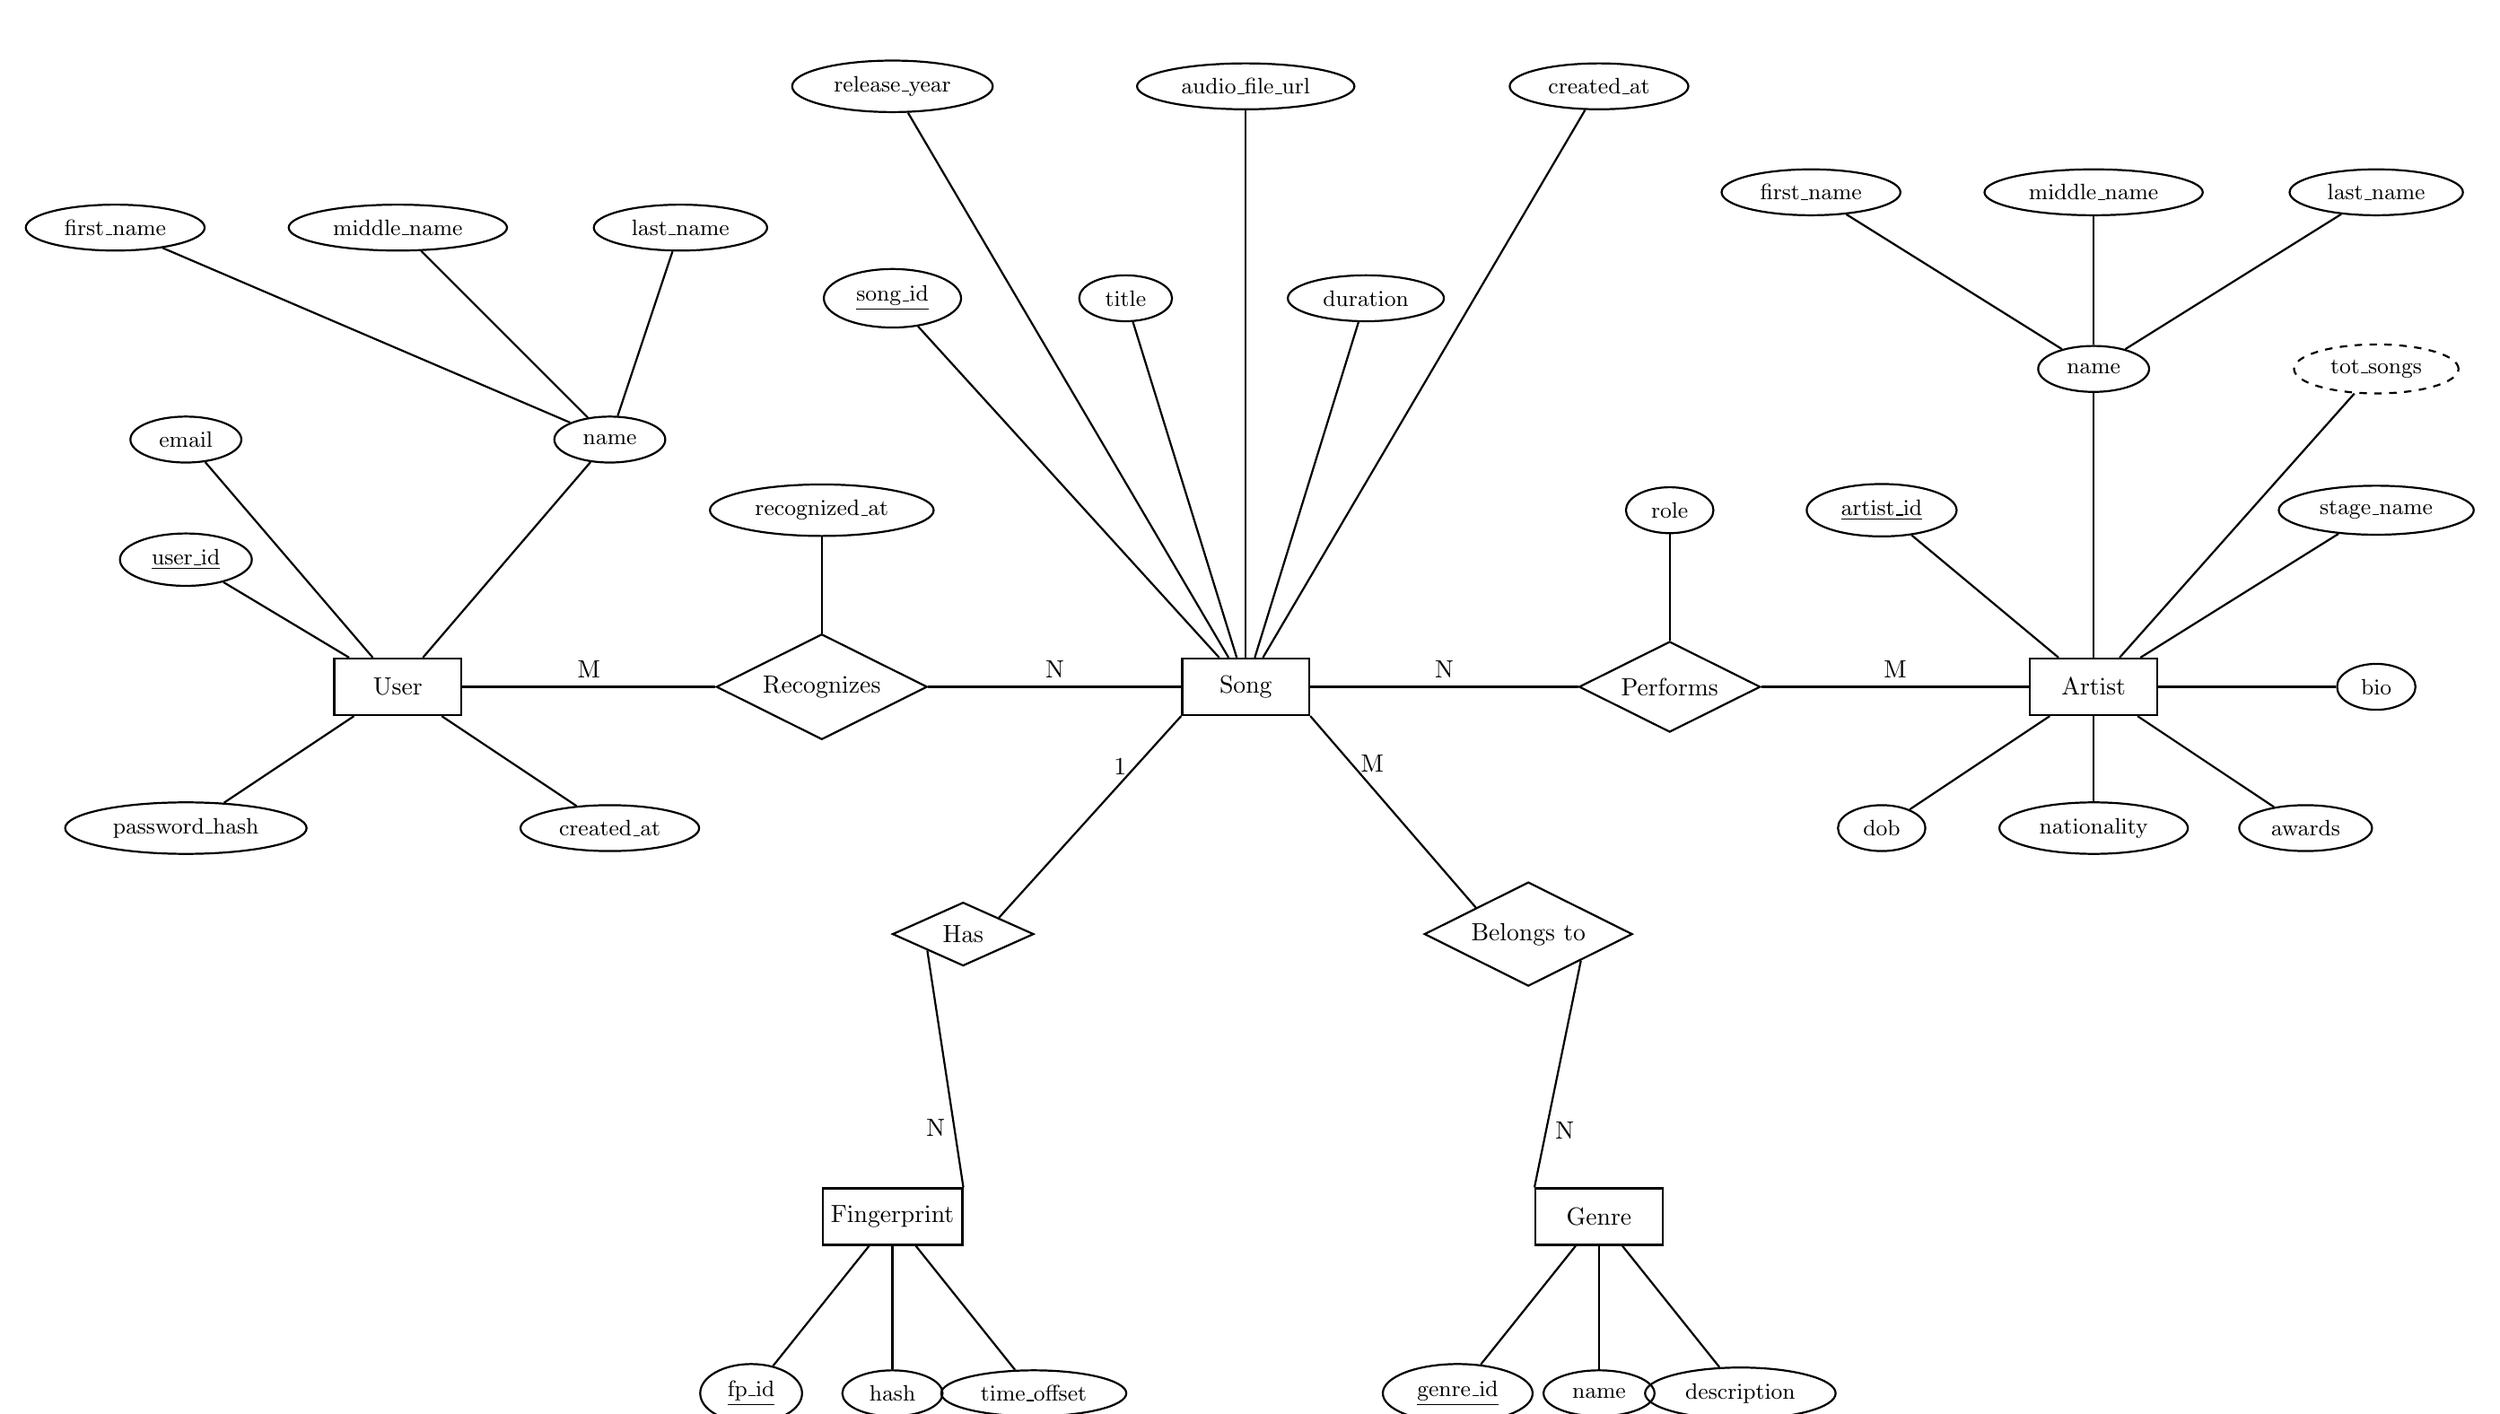
\begin{tikzpicture}[
    entity/.style={
        rectangle,
        draw=black,
        thick,
        minimum width=1.8cm,
        minimum height=0.8cm,
        font=\normalsize
    },
    relationship/.style={
        diamond,
        draw=black,
        thick,
        aspect=2,
        minimum width=2cm,
        minimum height=0.9cm,
        font=\normalsize
    },
    attribute/.style={
        ellipse,
        draw=black,
        thick,
        minimum height=0.65cm,
        inner xsep=5pt,
        font=\small
    },
    derived/.style={
        attribute,
        dashed
    },
    conn/.style={thick}
]

% =====================================================
% ENTITIES
% =====================================================

\node[entity] (User) at (-12,0) {User};
\node[entity] (Song) at (0,0) {Song};
\node[entity] (Artist) at (12,0) {Artist};

\node[entity] (Fingerprint) at (-5,-7.5) {Fingerprint};
\node[entity] (Genre) at (5,-7.5) {Genre};


% =====================================================
% USER ATTRIBUTES
% =====================================================

\node[attribute] (uid) at (-15,1.8)
    {\underline{user\_id}};

\node[attribute] (uemail) at (-15,3.5)
    {email};

\node[attribute] (uname) at (-9,3.5)
    {name};

\node[attribute] (upassword) at (-15,-2)
    {password\_hash};

\node[attribute] (ucreated) at (-9,-2)
    {created\_at};

% Composite name components

\node[attribute] (ufirst) at (-16,6.5)
    {first\_name};

\node[attribute] (umiddle) at (-12,6.5)
    {middle\_name};

\node[attribute] (ulast) at (-8,6.5)
    {last\_name};

\draw[conn] (User) -- (uid);
\draw[conn] (User) -- (uemail);
\draw[conn] (User) -- (uname);
\draw[conn] (User) -- (upassword);
\draw[conn] (User) -- (ucreated);

\draw[conn] (uname) -- (ufirst);
\draw[conn] (uname) -- (umiddle);
\draw[conn] (uname) -- (ulast);


% =====================================================
% SONG ATTRIBUTES
% =====================================================

% =====================================================
% SONG ATTRIBUTES - SPACED LAYOUT
% =====================================================

% First row
\node[attribute] (sid) at (-5,5.5)
    {\underline{song\_id}};

\node[attribute] (stitle) at (-1.7,5.5)
    {title};

\node[attribute] (sduration) at (1.7,5.5)
    {duration};

% Second row
\node[attribute] (syear) at (-5,8.5)
    {release\_year};

\node[attribute] (surl) at (0,8.5)
    {audio\_file\_url};

\node[attribute] (screated) at (5,8.5)
    {created\_at};

% Connections
\draw[conn] (Song) -- (sid);
\draw[conn] (Song) -- (stitle);
\draw[conn] (Song) -- (sduration);
\draw[conn] (Song) -- (syear);
\draw[conn] (Song) -- (surl);
\draw[conn] (Song) -- (screated);


% =====================================================
% ARTIST ATTRIBUTES
% =====================================================

\node[attribute] (aid) at (9,2.5)
    {\underline{artist\_id}};

\node[attribute] (aname) at (12,4.5)
    {name};

\node[attribute] (astage) at (16,2.5)
    {stage\_name};

\node[attribute] (afirst) at (8,7)
    {first\_name};

\node[attribute] (amiddle) at (12,7)
    {middle\_name};

\node[attribute] (alast) at (16,7)
    {last\_name};

\node[attribute] (adob) at (9,-2)
    {dob};

\node[attribute] (anationality) at (12,-2)
    {nationality};

\node[attribute] (aawards) at (15,-2)
    {awards};

\node[attribute] (abio) at (16,0)
    {bio};

\node[derived] (atotsongs) at (16,4.5)
    {tot\_songs};

\draw[conn] (Artist) -- (aid);
\draw[conn] (Artist) -- (aname);
\draw[conn] (Artist) -- (astage);
\draw[conn] (Artist) -- (adob);
\draw[conn] (Artist) -- (anationality);
\draw[conn] (Artist) -- (aawards);
\draw[conn] (Artist) -- (abio);
\draw[conn] (Artist) -- (atotsongs);

\draw[conn] (aname) -- (afirst);
\draw[conn] (aname) -- (amiddle);
\draw[conn] (aname) -- (alast);


% =====================================================
% FINGERPRINT ATTRIBUTES
% =====================================================

\node[attribute] (fid) at (-7,-10)
    {\underline{fp\_id}};

\node[attribute] (fhash) at (-5,-10)
    {hash};

\node[attribute] (foffset) at (-3,-10)
    {time\_offset};

\draw[conn] (Fingerprint) -- (fid);
\draw[conn] (Fingerprint) -- (fhash);
\draw[conn] (Fingerprint) -- (foffset);


% =====================================================
% GENRE ATTRIBUTES
% =====================================================

\node[attribute] (gid) at (3,-10)
    {\underline{genre\_id}};

\node[attribute] (gname) at (5,-10)
    {name};

\node[attribute] (gdescription) at (7,-10)
    {description};

\draw[conn] (Genre) -- (gid);
\draw[conn] (Genre) -- (gname);
\draw[conn] (Genre) -- (gdescription);


% =====================================================
% RELATIONSHIP DIAMONDS
% =====================================================

\node[relationship] (Recognizes) at (-6,0)
    {Recognizes};

\node[relationship] (Performs) at (6,0)
    {Performs};

\node[relationship] (Has) at (-4,-3.5)
    {Has};

\node[relationship] (Belongs) at (4,-3.5)
    {Belongs to};


% =====================================================
% USER -- RECOGNIZES -- SONG (M:N)
% =====================================================

\draw[conn] (User.east) --
    node[above]{M} (Recognizes.west);

\draw[conn] (Recognizes.east) --
    node[above]{N} (Song.west);

\node[attribute] (recognizedat) at (-6,2.5)
    {recognized\_at};

\draw[conn] (Recognizes) -- (recognizedat);


% =====================================================
% SONG -- PERFORMS -- ARTIST (M:N)
% =====================================================

\draw[conn] (Song.east) --
    node[above]{N} (Performs.west);

\draw[conn] (Performs.east) --
    node[above]{M} (Artist.west);

\node[attribute] (role) at (6,2.5)
    {role};

\draw[conn] (Performs) -- (role);


% =====================================================
% SONG -- HAS -- FINGERPRINT (1:N)
% =====================================================

\draw[conn] (Song.south west) --
    node[left, near start]{1} (Has.north east);

\draw[conn] (Has.south west) --
    node[left, near end]{N} (Fingerprint.north east);


% =====================================================
% SONG -- BELONGS TO -- GENRE (M:N)
% =====================================================

\draw[conn] (Song.south east) --
    node[right, near start]{M} (Belongs.north west);

\draw[conn] (Belongs.south east) --
    node[right, near end]{N} (Genre.north west);

\end{tikzpicture}%
}

\caption{Conceptual Entity-Relationship Diagram of VibeCheck}
\label{fig:vibecheck-er}

\end{figure}
\end{landscape}
%% ------------------------------------------------------------------ 5
\section{Relational Schemas Obtained from ER}

\subsection{Mapping rules applied}

\begin{enumerate}
  \item Each strong entity becomes a relation whose attributes are the simple attributes of the entity. A composite attribute is replaced by its components (\cl{name} becomes \cl{first_name}, \cl{middle_name}, \cl{last_name}). The key attribute becomes the primary key.
  \item Each M:N relationship becomes a separate relation containing the primary keys of both participating entities (as foreign keys, together forming the primary key) plus the attributes of the relationship.
  \item Each 1:N relationship is represented by adding the primary key of the ``one'' side to the ``many'' side as a foreign key.
  \item The derived attribute \cl{tot_songs} is stored as an ordinary column and kept correct by a trigger (see Section~7.4).
\end{enumerate}

\subsection{Relations}

Primary keys are underlined; foreign keys are listed below the relations.

\begin{itemize}[leftmargin=*,itemsep=4pt]
  \item \textbf{Users}(\pk{user_id}, \cl{first_name}, \cl{middle_name}, \cl{last_name}, \cl{email}, \cl{password_hash}, \cl{created_at})
  \item \textbf{Artists}(\pk{artist_id}, \cl{first_name}, \cl{middle_name}, \cl{last_name}, \cl{stage_name}, \cl{dob}, \cl{nationality}, \cl{tot_songs}, \cl{awards}, \cl{bio})
  \item \textbf{Genres}(\pk{genre_id}, \cl{name}, \cl{description})
  \item \textbf{Songs}(\pk{song_id}, \cl{title}, \cl{duration}, \cl{release_year}, \cl{created_at})
  \item \textbf{Song\_Artists}(\pk{song_id}, \pk{artist_id}, \cl{role})
  \item \textbf{Song\_Genres}(\pk{song_id}, \pk{genre_id})
  \item \textbf{Fingerprints}(\pk{fp_id}, \cl{song_id}, \cl{hash}, \cl{time_offset})
  \item \textbf{History}(\pk{history_id}, \cl{user_id}, \cl{song_id}, \cl{recognized_at})
\end{itemize}

\subsection{Foreign keys}

All foreign keys are declared with \texttt{ON DELETE CASCADE}, so deleting a parent row removes its dependent rows.

\begin{center}
\begin{tabular}{|l|l|l|}
\hline
\textbf{Child relation} & \textbf{Foreign key} & \textbf{References} \\
\hline
Song\_Artists & \cl{song_id} & Songs(\cl{song_id}) \\
\hline
Song\_Artists & \cl{artist_id} & Artists(\cl{artist_id}) \\
\hline
Song\_Genres & \cl{song_id} & Songs(\cl{song_id}) \\
\hline
Song\_Genres & \cl{genre_id} & Genres(\cl{genre_id}) \\
\hline
Fingerprints & \cl{song_id} & Songs(\cl{song_id}) \\
\hline
History & \cl{user_id} & Users(\cl{user_id}) \\
\hline
History & \cl{song_id} & Songs(\cl{song_id}) \\
\hline
\end{tabular}
\end{center}

\subsection{Data types and constraints}

\begin{longtable}{|p{3.2cm}|p{3.4cm}|p{9.2cm}|}
\hline
\textbf{Attribute} & \textbf{Data type} & \textbf{Constraints} \\
\hline
\endfirsthead

\hline
\textbf{Attribute} & \textbf{Data type} & \textbf{Constraints} \\
\hline
\endhead

\multicolumn{3}{|l|}{\textbf{Users}} \\
\hline
\cl{user_id} & \cl{SERIAL} & Primary key, auto-increment \\
\hline
\cl{first_name} & \cl{VARCHAR(50)} & NOT NULL \\
\hline
\cl{middle_name} & \cl{VARCHAR(50)} & optional \\
\hline
\cl{last_name} & \cl{VARCHAR(50)} & optional \\
\hline
\cl{email} & \cl{VARCHAR(255)} & UNIQUE, NOT NULL, CHECK for a valid e-mail pattern \\
\hline
\cl{password_hash} & \cl{VARCHAR(255)} & NOT NULL \\
\hline
\cl{created_at} & \cl{TIMESTAMP} & DEFAULT current time \\
\hline

\multicolumn{3}{|l|}{\textbf{Artists}} \\
\hline
\cl{artist_id} & \cl{SERIAL} & Primary key, auto-increment \\
\hline
\cl{first_name}, \cl{middle_name}, \cl{last_name} & \cl{VARCHAR(50)} & optional \\
\hline
\cl{stage_name} & \cl{VARCHAR(100)} & UNIQUE, NOT NULL \\
\hline
\cl{dob} & \cl{DATE} & CHECK date of birth is in the past \\
\hline
\cl{nationality} & \cl{VARCHAR(50)} & optional \\
\hline
\cl{tot_songs} & \cl{INT} & DEFAULT 0, CHECK $\geq 0$ \\
\hline
\cl{awards}, \cl{bio} & \cl{TEXT} & optional \\
\hline

\multicolumn{3}{|l|}{\textbf{Genres}} \\
\hline
\cl{genre_id} & \cl{SERIAL} & Primary key, auto-increment \\
\hline
\cl{name} & \cl{VARCHAR(50)} & UNIQUE, NOT NULL \\
\hline
\cl{description} & \cl{TEXT} & optional \\
\hline

\multicolumn{3}{|l|}{\textbf{Songs}} \\
\hline
\cl{song_id} & \cl{SERIAL} & Primary key, auto-increment \\
\hline
\cl{title} & \cl{VARCHAR(150)} & NOT NULL \\
\hline
\cl{duration} & \cl{INT} & NOT NULL, CHECK $> 0$ (seconds) \\
\hline
\cl{release_year} & \cl{INT} & CHECK $\geq 1900$ \\

\hline
\cl{created_at} & \cl{TIMESTAMP} & DEFAULT current time \\
\hline

\multicolumn{3}{|l|}{\textbf{Song\_Artists}} \\
\hline
\cl{song_id} & \cl{INT} & Part of primary key, FK to Songs, ON DELETE CASCADE \\
\hline
\cl{artist_id} & \cl{INT} & Part of primary key, FK to Artists, ON DELETE CASCADE \\
\hline
\cl{role} & \cl{VARCHAR(50)} & DEFAULT \texttt{'Primary'}, CHECK in (Primary, Featured, Producer) \\
\hline

\multicolumn{3}{|l|}{\textbf{Song\_Genres}} \\
\hline
\cl{song_id} & \cl{INT} & Part of primary key, FK to Songs, ON DELETE CASCADE \\
\hline
\cl{genre_id} & \cl{INT} & Part of primary key, FK to Genres, ON DELETE CASCADE \\
\hline

\multicolumn{3}{|l|}{\textbf{Fingerprints}} \\
\hline
\cl{fp_id} & \cl{BIGSERIAL} & Primary key, auto-increment \\
\hline
\cl{song_id} & \cl{INT} & NOT NULL, FK to Songs, ON DELETE CASCADE, indexed \\
\hline
\cl{hash} & \cl{BIGINT} & NOT NULL, B-Tree index \\
\hline
\cl{time_offset} & \cl{INT} & NOT NULL, CHECK $\geq 0$ (frame number in the song) \\
\hline

\multicolumn{3}{|l|}{\textbf{History}} \\
\hline
\cl{history_id} & \cl{BIGSERIAL} & Primary key, auto-increment \\
\hline
\cl{user_id} & \cl{INT} & NOT NULL, FK to Users, ON DELETE CASCADE \\
\hline
\cl{song_id} & \cl{INT} & NOT NULL, FK to Songs, ON DELETE CASCADE \\
\hline
\cl{recognized_at} & \cl{TIMESTAMP} & DEFAULT current time; index on (\cl{user_id}, \cl{recognized_at} descending) \\
\hline
\end{longtable}
%% ------------------------------------------------------------------ 6
\section{Functional Dependencies on Each Table}

The following functional dependencies must hold in every valid state of the database. They follow from the meaning of the attributes and from the declared keys. Right-hand sides written as ``all other attributes'' list every non-key attribute of the table.

\begin{longtable}{|p{2.4cm}|p{3.2cm}|p{10.0cm}|}
\hline
\textbf{Relation} & \textbf{Candidate key(s)} & \textbf{Functional dependencies} \\
\hline
\endfirsthead

\hline
\textbf{Relation} & \textbf{Candidate key(s)} & \textbf{Functional dependencies} \\
\hline
\endhead

Users & \cl{user_id}; \cl{email} &
\cl{user_id} $\rightarrow$ \cl{first_name}, \cl{middle_name}, \cl{last_name}, \cl{email}, \cl{password_hash}, \cl{created_at}\newline
\cl{email} $\rightarrow$ \cl{user_id} \\
\hline

Artists & \cl{artist_id}; \cl{stage_name} &
\cl{artist_id} $\rightarrow$ \cl{first_name}, \cl{middle_name}, \cl{last_name}, \cl{stage_name}, \cl{dob}, \cl{nationality}, \cl{tot_songs}, \cl{awards}, \cl{bio}\newline
\cl{stage_name} $\rightarrow$ \cl{artist_id} \\
\hline

Genres & \cl{genre_id}; \cl{name} &
\cl{genre_id} $\rightarrow$ \cl{name}, \cl{description}\newline
\cl{name} $\rightarrow$ \cl{genre_id} \\
\hline

Songs & \cl{song_id} &
\cl{song_id} $\rightarrow$ \cl{title}, \cl{duration}, \cl{release_year}, \cl{audio_file_url}, \cl{created_at} \\
\hline

Song\_Artists & (\cl{song_id}, \cl{artist_id}) &
(\cl{song_id}, \cl{artist_id}) $\rightarrow$ \cl{role} \\
\hline

Song\_Genres & (\cl{song_id}, \cl{genre_id}) &
Only the trivial dependencies; the whole row is the key \\
\hline

Fingerprints & \cl{fp_id} &
\cl{fp_id} $\rightarrow$ \cl{song_id}, \cl{hash}, \cl{time_offset} \\
\hline

History & \cl{history_id} &
\cl{history_id} $\rightarrow$ \cl{user_id}, \cl{song_id}, \cl{recognized_at} \\
\hline
\end{longtable}

\textbf{Assumptions.} Two different songs may have the same title, so \cl{title} does not determine \cl{song_id}. Likewise a hash value can occur in many songs and at many times, so \cl{hash} determines nothing else, and \cl{role} depends on the combination of a song and an artist, not on either alone. Different users can recognize the same song, and one user can recognize it repeatedly, so \cl{user_id} and \cl{song_id} together do not determine \cl{history_id}.

%% ------------------------------------------------------------------ 7
\section{Normalization up to 3NF}

\subsection{Definitions used}

\begin{itemize}
  \item \textbf{1NF:} all attribute values are atomic; there are no repeating groups or multi-valued columns.
  \item \textbf{2NF:} the relation is in 1NF and no non-prime attribute depends on only part of a composite candidate key.
  \item \textbf{3NF:} the relation is in 2NF and, for every non-trivial dependency $X \rightarrow A$, either $X$ is a superkey or $A$ is a prime attribute (so no non-prime attribute depends transitively on a key).
\end{itemize}

\subsection{How the design was reached}

The design was reached in stages, starting from flat tables that hold everything. For every stage the relations, their keys and the dependencies used are listed; primary keys are underlined. Only the attributes needed to show each step are included, and the remaining columns of Users, Artists, Songs and so on are added in the final schema.

\subsubsection*{Stage 0: unnormalized}

All information about a song is kept in one table, with repeating groups (written in braces):
\begin{quote}
\textbf{SongInfo0}(\pk{song_id}, \cl{title}, \cl{duration}, \cl{release_year}, \{\cl{artist_id}, \cl{stage_name}, \cl{nationality}, \cl{role}\}, \{\cl{genre_id}, \cl{genre_name}\})
\end{quote}
A song can have several artists and several genres, so one row would have to hold a list of artists and a list of genres. This is not even in 1NF.

\subsubsection*{Stage 1: first normal form (1NF)}

Repeating groups are removed by giving every combination of song, artist and genre its own row, so all values become atomic. The recognition side of the system is also kept as flat tables at this stage:
\begin{itemize}[leftmargin=*,itemsep=4pt]
  \item \textbf{SongInfo}(\pk{song_id}, \pk{artist_id}, \pk{genre_id}, \cl{title}, \cl{duration}, \cl{release_year}, \cl{stage_name}, \cl{nationality}, \cl{role}, \cl{genre_name})
  \item \textbf{RecognitionLog}(\pk{history_id}, \cl{user_id}, \cl{first_name}, \cl{email}, \cl{song_id}, \cl{title}, \cl{recognized_at})
  \item \textbf{FingerprintLog}(\pk{fp_id}, \cl{song_id}, \cl{title}, \cl{hash}, \cl{time_offset})
\end{itemize}
The dependencies that hold are:
\begin{itemize}[leftmargin=*,itemsep=2pt]
  \item \cl{song_id} $\rightarrow$ \cl{title}, \cl{duration}, \cl{release_year}
  \item \cl{artist_id} $\rightarrow$ \cl{stage_name}, \cl{nationality}
  \item (\cl{song_id}, \cl{artist_id}) $\rightarrow$ \cl{role}
  \item \cl{genre_id} $\rightarrow$ \cl{genre_name}
  \item \cl{history_id} $\rightarrow$ \cl{user_id}, \cl{song_id}, \cl{recognized_at}; \cl{user_id} $\rightarrow$ \cl{first_name}, \cl{email}; \cl{song_id} $\rightarrow$ \cl{title}
  \item \cl{fp_id} $\rightarrow$ \cl{song_id}, \cl{hash}, \cl{time_offset}; \cl{song_id} $\rightarrow$ \cl{title}
\end{itemize}
\textbf{Problems:} the title and duration of a song are repeated for every artist and genre combination, an artist cannot be stored before having a song, and deleting the last song of an artist would erase the artist's data.

\subsubsection*{Stage 2: second normal form (2NF)}

In SongInfo the key has three attributes, but \cl{title}, \cl{duration}, \cl{release_year}, \cl{stage_name}, \cl{nationality} and \cl{genre_name} each depend on only a part of the key, and \cl{role} depends on two of the three. These partial dependencies are removed by splitting SongInfo into one relation per dependency:
\begin{itemize}[leftmargin=*,itemsep=4pt]
  \item \textbf{Song}(\pk{song_id}, \cl{title}, \cl{duration}, \cl{release_year})
  \item \textbf{Artist}(\pk{artist_id}, \cl{stage_name}, \cl{nationality})
  \item \textbf{Genre}(\pk{genre_id}, \cl{genre_name})
  \item \textbf{SongArtist}(\pk{song_id}, \pk{artist_id}, \cl{role})
  \item \textbf{SongGenre}(\pk{song_id}, \pk{genre_id})
  \item \textbf{RecognitionLog}(\pk{history_id}, \cl{user_id}, \cl{first_name}, \cl{email}, \cl{song_id}, \cl{title}, \cl{recognized_at}) \quad (unchanged)
  \item \textbf{FingerprintLog}(\pk{fp_id}, \cl{song_id}, \cl{title}, \cl{hash}, \cl{time_offset}) \quad (unchanged)
\end{itemize}
Now every non-key attribute depends on the whole key of its relation. RecognitionLog and FingerprintLog have single-attribute keys, so they cannot have partial dependencies and are already in 2NF.

\subsubsection*{Stage 3: third normal form (3NF)}

RecognitionLog and FingerprintLog are in 2NF but not in 3NF, because they contain transitive dependencies:
\begin{itemize}[leftmargin=*,itemsep=2pt]
  \item \cl{history_id} $\rightarrow$ \cl{user_id} $\rightarrow$ \cl{first_name}, \cl{email}
  \item \cl{history_id} $\rightarrow$ \cl{song_id} $\rightarrow$ \cl{title}
  \item \cl{fp_id} $\rightarrow$ \cl{song_id} $\rightarrow$ \cl{title}
\end{itemize}
If a user changed an e-mail address, every one of their history rows would have to change, and the title of a song would be repeated in every fingerprint row of that song (tens of thousands of times). The transitive dependencies are removed by keeping only the foreign key and moving the other attributes to the relation that owns them:
\begin{itemize}[leftmargin=*,itemsep=4pt]
  \item \textbf{History}(\pk{history_id}, \cl{user_id}, \cl{song_id}, \cl{recognized_at})
  \item \textbf{Users}(\pk{user_id}, \cl{first_name}, \cl{email}, \ldots)
  \item \textbf{Fingerprints}(\pk{fp_id}, \cl{song_id}, \cl{hash}, \cl{time_offset})
  \item \textbf{Songs}(\pk{song_id}, \cl{title}, \cl{duration}, \cl{release_year}, \ldots) \quad (the Song relation of Stage 2)
\end{itemize}
Together with Artists, Genres, Song\_Artists and Song\_Genres from Stage 2 (with their remaining columns added), these are the eight relations of Section~5.

\begin{center}
\begin{tabular}{|p{3.6cm}|p{12.2cm}|}
\hline
\textbf{Stage} & \textbf{Relations after the stage} \\
\hline
0 (unnormalized) & SongInfo0 \\
\hline
1 (1NF) & SongInfo, RecognitionLog, FingerprintLog \\
\hline
2 (2NF) & Song, Artist, Genre, SongArtist, SongGenre, RecognitionLog, FingerprintLog \\
\hline
3 (3NF) & Users, Artists, Genres, Songs, Song\_Artists, Song\_Genres, Fingerprints, History \\
\hline
\end{tabular}
\end{center}

\subsection{Normal form of each relation}
\begin{longtable}{|p{2.0cm}|p{0.8cm}|p{0.8cm}|p{0.8cm}|p{8.8cm}|}
\hline
\textbf{Relation} & \textbf{1NF} & \textbf{2NF} & \textbf{3NF} & \textbf{Justification} \
\hline
\endfirsthead

\hline
\textbf{Relation} & \textbf{1NF} & \textbf{2NF} & \textbf{3NF} & \textbf{Justification} \
\hline
\endhead

Users & Yes & Yes & Yes & All values are atomic (the name is split into three columns). The key \cl{user_id} is a single attribute, so there are no partial dependencies. Every determinant (\cl{user_id}, \cl{email}) is a candidate key. \
\hline

Artists & Yes & Yes & Yes & Single-attribute key; the only determinants are \cl{artist_id} and \cl{stage_name}, both candidate keys. No non-prime attribute determines another. \
\hline

Genres & Yes & Yes & Yes & The determinants \cl{genre_id} and \cl{name} are both candidate keys. \
\hline

Songs & Yes & Yes & Yes & The only determinant is the key \cl{song_id}; artist and genre data are not stored here. \
\hline

Song\_Artists & Yes & Yes & Yes & The only non-key attribute, \cl{role}, depends on the whole key (\cl{song_id}, \cl{artist_id}), not on a part of it. \
\hline

Song\_Genres & Yes & Yes & Yes & All attributes belong to the key, so there are no non-prime attributes. \
\hline

Fingerprints & Yes & Yes & Yes & Single-attribute key \cl{fp_id}; \cl{song_id}, \cl{hash}, and \cl{time_offset} describe the fingerprint row. \
\hline

History & Yes & Yes & Yes & Single-attribute key \cl{history_id}; \cl{user_id}, \cl{song_id}, and \cl{recognized_at} describe one recognition event and do not determine each other. \
\hline
\end{longtable}

In each relation every determinant is a candidate key, so all eight relations are also in Boyce--Codd Normal Form.

\subsection{Controlled redundancy: \texttt{tot\_songs}}

The column \cl{Artists.tot_songs} is derived, because it equals the number of rows of Song\_Artists for that artist. Storing it is a deliberate choice that makes it cheap to display an artist's song count without a join and aggregation. To prevent the stored value from becoming inconsistent, two triggers on Song\_Artists increase the count after an insert and decrease it after a delete (never below zero). The value is therefore never edited by hand, and the design stays consistent while avoiding repeated counting.

\subsection{Conclusion}

All eight tables satisfy 1NF, 2NF and 3NF (and BCNF). Each fact is stored once, many-to-many relationships are resolved through the linking tables Song\_Artists and Song\_Genres, and consistency is enforced by keys, check constraints, cascading foreign keys and a trigger.

%% ------------------------------------------------------------------ appendix
\appendix
\section{Database Objects Used by the Application}

\subsection{Indexes}
\begin{lstlisting}
CREATE INDEX idx_fingerprints_hash ON Fingerprints(hash);
CREATE INDEX idx_fingerprints_song ON Fingerprints(song_id);
CREATE INDEX idx_history_user ON History(user_id, recognized_at DESC);
\end{lstlisting}
The index on \cl{hash} makes the matching query \texttt{WHERE hash = ANY(...)} an index scan instead of a full table scan. The history index serves the query that lists a user's latest recognitions.

\subsection{Trigger to keep \texttt{tot\_songs} correct}
\begin{lstlisting}
CREATE OR REPLACE FUNCTION update_artist_song_count() RETURNS TRIGGER AS $$
BEGIN
  IF TG_OP = 'INSERT' THEN
    UPDATE Artists SET tot_songs = tot_songs + 1 WHERE artist_id = NEW.artist_id;
    RETURN NEW;
  ELSIF TG_OP = 'DELETE' THEN
    UPDATE Artists SET tot_songs = GREATEST(tot_songs - 1, 0) WHERE artist_id = OLD.artist_id;
    RETURN OLD;
  END IF;
  RETURN NULL;
END; $$ LANGUAGE plpgsql;

CREATE TRIGGER trg_increment_tot_songs AFTER INSERT ON Song_Artists
  FOR EACH ROW EXECUTE FUNCTION update_artist_song_count();
CREATE TRIGGER trg_decrement_tot_songs AFTER DELETE ON Song_Artists
  FOR EACH ROW EXECUTE FUNCTION update_artist_song_count();
\end{lstlisting}

\subsection{Stored function to log a recognition}
\begin{lstlisting}
CREATE OR REPLACE FUNCTION log_recognition(p_user INT, p_song INT) RETURNS BIGINT AS $$
DECLARE new_id BIGINT;
BEGIN
  INSERT INTO History(user_id, song_id) VALUES (p_user, p_song) RETURNING history_id INTO new_id;
  RETURN new_id;
END; $$ LANGUAGE plpgsql;
\end{lstlisting}
The API calls this function in the same transaction in which it reads the matched song, so the history entry and the response are consistent.

\subsection{Views}
\begin{lstlisting}
CREATE OR REPLACE VIEW v_song_details AS
SELECT s.song_id, s.title, s.duration, s.release_year,
       COALESCE(string_agg(DISTINCT a.stage_name, ', '), 'Unknown') AS artists,
       COALESCE(string_agg(DISTINCT g.name, ' / '), 'Unclassified') AS genres
FROM Songs s
LEFT JOIN Song_Artists sa ON sa.song_id = s.song_id
LEFT JOIN Artists a ON a.artist_id = sa.artist_id
LEFT JOIN Song_Genres sg ON sg.song_id = s.song_id
LEFT JOIN Genres g ON g.genre_id = sg.genre_id
GROUP BY s.song_id;

CREATE OR REPLACE VIEW v_user_history AS
SELECT h.history_id, h.user_id, h.recognized_at, d.*
FROM History h JOIN v_song_details d ON d.song_id = h.song_id;
\end{lstlisting}

\newpage
\subsection{Sample queries for demonstration}
\begin{lstlisting}
EXPLAIN ANALYZE SELECT * FROM Fingerprints WHERE hash = 123;
SELECT * FROM v_user_history;
SELECT stage_name, tot_songs FROM Artists;
\end{lstlisting}

\end{document}
